\documentclass[a4paper, 12pt]{scrreprt}

\usepackage[automark,headsepline,ilines,komastyle,autooneside]{scrpage2} 
\usepackage[left=1.5cm,right=2.5cm,top=2cm,bottom=2cm,includeheadfoot]{geometry}
\usepackage[ngerman]{babel}
\usepackage[T1]{fontenc} 
\usepackage[utf8]{inputenc}
%% \usepackage{inputenc}
\usepackage[osf,sc]{mathpazo}
\usepackage{lmodern, hfoldsty, charter}
%% \usepackage[scaled=.95]{helvet}
%% \usepackage[usenames,dvipsnames]{xcolor}
%% \usepackage{framed}
\usepackage{hyperref} 
\usepackage{graphicx}
\usepackage{makeidx}
\usepackage{color} 
\usepackage{float}
\usepackage{listings}
\usepackage{marvosym}
%% \usepackage{paralist}
\usepackage[onehalfspacing]{setspace}

\makeindex

\pagestyle{scrheadings}

\makeatother

\begin{document}
\pagenumbering{roman}
\thispagestyle{empty}
\begin{figure}[t]
 \centering
 
\includegraphics[width=0.6\textwidth]{pictures/ostfaliaLogo}
\end{figure}

\begin{verbatim}


\end{verbatim}

\begin{center}
\Large{Ostfalia Hochschule für angewandte Wissenschaften}\\
\Large{Wolfenbüttel}\\
\end{center}

\begin{center}
\Large{Fakultät Informatik}
\end{center}

\begin{verbatim}


\end{verbatim}

\begin{center}
\doublespacing
\textbf{\LARGE{Hausarbeit}}\\
\singlespacing

\begin{verbatim}

\end{verbatim}

\textbf{{~im Studiengang Informatik~-~Fach Gespräch und Verhandlungsführung~}}

\end{center}

\begin{verbatim}

\end{verbatim}

\begin{center}
Boris Nguema B. 70423512 \Letter  b.nguemabekale@ostfalia.de\\
Valentin Gelhorn 70373477 \Letter  va.gelhorn@ostfalia.de\\
Wladimir David Zakrevskyy 70351576 \Letter  w.zakrevskyy@ostfalia.de\\
\end{center}
\begin{center}
\textbf{Version vom:}\today\\
\textbf{Betreuer:} Norbert Köhler \Letter  nhk@nhk-consult.de\\
\end{center}

\thispagestyle{empty}
\clearpage

\renewcommand*{\chapterpagestyle}{empty}
\thispagestyle{empty}
\tableofcontents

\thispagestyle{empty}
\clearpage

\pagenumbering{arabic}
\setcounter{page}{1}
 
\chapter{Einführung}
In dieser Arbeit wird Anhand einer skizierten Situation eine Verhalndung nach dem "`Harvard-Konzept des Sachgerechten Verhandelns"'\cite{hk} weiter
HKSV bearbeitet. Die Einführungskapiteln werden ein kurzen Überblick geben über die Aufbau von HKSV\cite{hk} geben. Danach wird die Situtation
Analysiert anhand von Interessen von Parteien, folgend von entwickelten Entscheidungsmöglichkeiten (Optionen) und abschließend werden noch weitere Alternativen für Einigung
der Parteien vorgestellt. Fazit dieser Arbeit wird ein Überblick und die Ergebnise vorstellen.
\section{Harvard-Konzept des Sachgerechten Verhandelns\cite{hk}}
Der nachfolgend dargestelltes Bild zeigt die Aufbau von HKSV\cite{hk}.
\begin{figure}[hb]
\centering
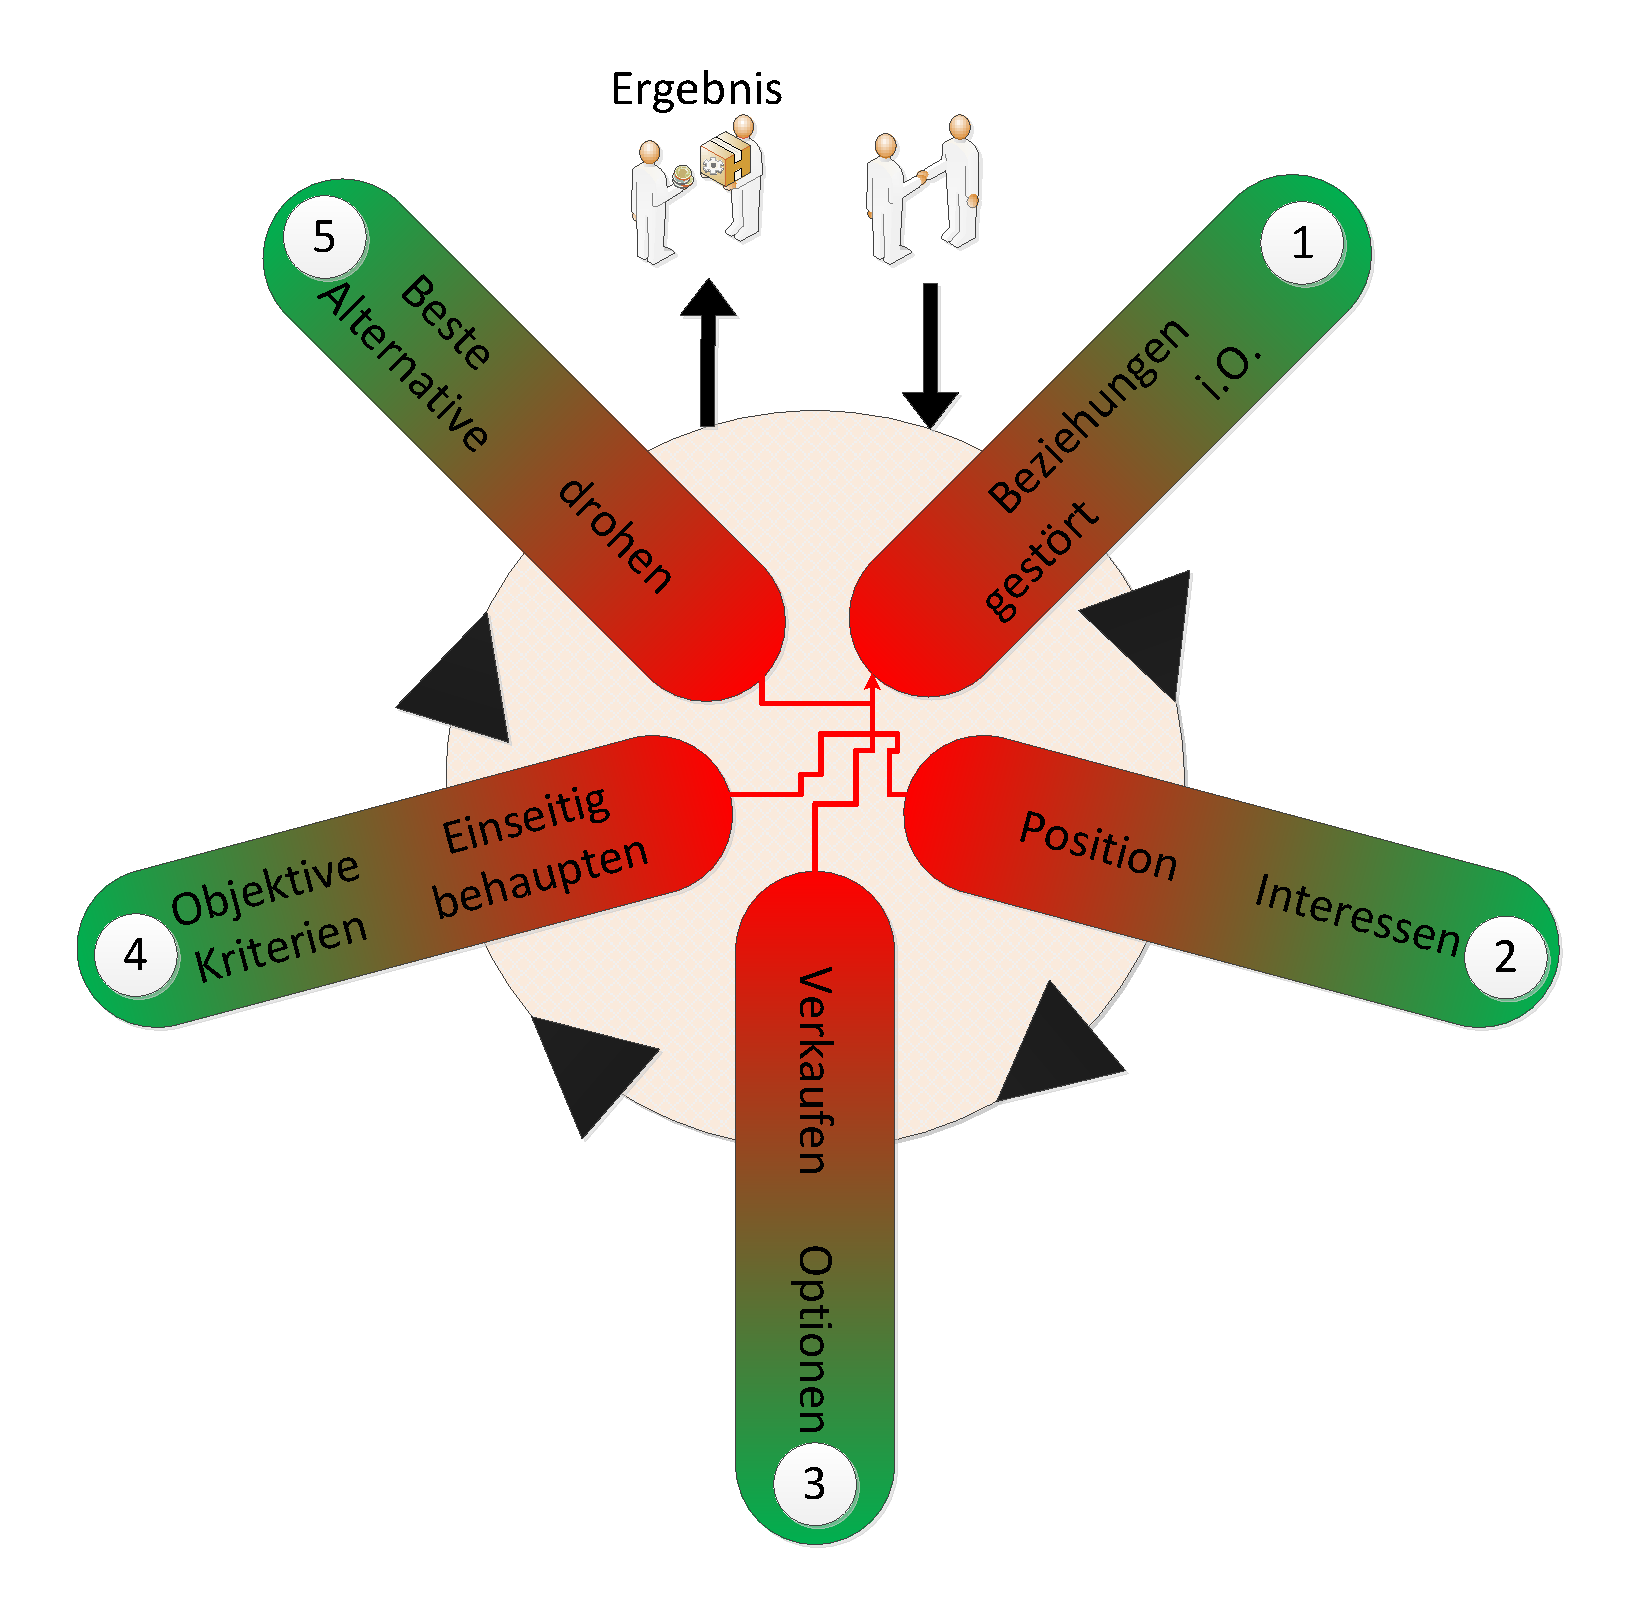
\includegraphics[width=0.4\paperwidth]{pictures/Harvard1}
\caption{Harvard-Konzept des Sachgerechten Verhandelns}
\end{figure}
Es sind die fünf Aspekte des Verhandelns zu erkennen, diese Beschreibt folgende Tabelle genauer. Die Punkte die in Bild mit Zahlen markiert sind
werden mit Stichwörtern markiert. Es wird verzichtet auf die genaueren Beschreibungen, da dies die Rahmen dieser Arbeit sprengen wird.
\begin{table}[h]
\begin{center}
\begin{tabular}{|l|l|l|}\hline
\textbf{Nummer} & \textbf{Name} & \textbf{Beschreibung} \\
\hline\hline
1 & Beziehungen & Trennung von Person und Sache \\
\hline
2 & Position vs Interessen & Interessenkonflikte, gemeinsame Interessen \\
\hline
3 & Verkaufen vs Optionen & Kreativität bei Lösungsstrategien \\
\hline
4 & Objektive Kriterien vs Behauptung & Ursachen, Standards, Werte \\
\hline
5 & Alternativen vs Drohungen & Alternativen für alle Beteiligten \\
\hline
\end{tabular}
\caption{Beschreibung von HKSV}
\label{tab:beschreibungHKSV}
\end{center}
\end{table}
\newpage
\chapter{Analyse}
Der Autor ist der Abteilungsleiter der WEK.
\section{Beteiligte Verhandlungsparteien}
	
\begin{itemize}
	\item Wolfsburger Ersatzkasse (WEK)
    	\subitem Vorstand der WEK
    	\subitem Abteilungsleiter
		\subitem Mitglieder der WEK
		\subitem zahlreiche Vertragspartner der WEK
    
	\item Dr. Kneip in folgenden Funktionen
		\subitem Bürgermeister des Kurortes Bad Fünfquelle
		\subitem Geschäftsführer Bad Fünfquell Kurbetriebs GmbH
    
    \item Bank
    \item Presse
    \item Stadtrat
	\item Gemeinderat 
    
    indirekt:
	\item Bürger	
	\item Mitarbeiter
\end{itemize}

\smallskip \textbf{Wolfsburger Ersatzkasse (WEK)} \\
\smallskip \textbf{Dr. Kneip} \\
\smallskip \textbf{Stadtrat / Opposition} \\
\smallskip \textbf{Presse} \\
\smallskip \textbf{Gemeinderat} \\
\smallskip \textbf{Bürger} \\
\smallskip \textbf{Mitarbeiter} \\

\smallskip \textbf{- Interessen und persönliche Motive beteiligter Parteien -} \\
\smallskip \textbf{Wolfsburger Ersatzkasse (WEK)} \\
\smallskip \textbf{Dr. Kneip} \\
\smallskip \textbf{Stadtrat / Opposition} \\
\smallskip \textbf{Presse} \\
\smallskip \textbf{Gemeinderat} \\
\smallskip \textbf{Bürger} \\
\smallskip \textbf{Mitarbeiter} \\

\smallskip \textbf{- Gewichtung der Interessen -} \\
\smallskip \textbf{Wolfsburger Ersatzkasse (WEK)} \\
\smallskip \textbf{Dr. Kneip} \\
\smallskip \textbf{Stadtrat / Opposition} \\
\smallskip \textbf{Presse} \\
\smallskip \textbf{Gemeinderat} \\
\smallskip \textbf{Bürger} \\
\smallskip \textbf{Mitarbeiter} \\

\section{Fazit der Analyse}
\newpage
\chapter{Task2}
\section{Task 2}
\newpage
\chapter{Task3}
\section{Task 3}
\newpage
\chapter{Fazit} 

\newpage

\appendix
\chapter{Anhang}
\section{Anhang A}

\addcontentsline{toc}{chapter}{Literaturverzeichnis}
% Non-BibTeX users please use
\begin{thebibliography}{99.}

\bibitem{hk} Fisher Roger und Willian Ury, Das Harvard-Konzept. Sachgerecht verhandeln-erfolgreich verhandeln, Frankfurt am Main, 1984
\bibitem{nk} Norbert Köhler, HIER KOMMT DAS BILD, Wolfenbüttel/Ostfalia, 2015

\end{thebibliography}

\end{document}